% !TEX TS-program = xelatex
\documentclass[12pt]{article}

\usepackage[margin=2cm]{geometry}
\usepackage{colortbl}
\usepackage{comment}
\usepackage{caption}
\usepackage{subcaption}
\usepackage{mathptmx}
\usepackage{nicefrac}
\usepackage{authblk}


\usepackage{times}
\usepackage{lineno}
\usepackage[round]{natbib}
\makeatletter
\renewcommand{\@biblabel}[1]{#1.}
\makeatother

\usepackage{graphicx}
\usepackage{amsmath}
\usepackage{xcolor}

\usepackage{url}
\urlstyle{same}

\usepackage[small,compact]{titlesec}

%\titleformat{\section} {\vspace{24pt}\bf\sffamily\MakeUppercase}{\thesection} {0pt} {}
\titleformat{\section} {\vspace{12pt}\bf\large}{S\thesection\ }{0pt}{}
\titleformat{\subsection} {\vspace{6pt}\bf}{\thesubsection} {0pt} {\vspace{-2pt}}
\titleformat{\subsubsection} [runin] {\bf}{\thesubsubsection} {12pt} {}

\definecolor{badpatcol}{HTML}{FF6666}
\newcommand{\badpat}[1]{\rowcolor{badpatcol}#1}

\captionsetup[subfigure]{width=0.9\textwidth}

\newcommand{\high}[1]{{\textcolor{badpatcol} #1}} 
 
\begin{document}

\title{Supplementary Materials \\ Blind dating: a phylogenetic approach to determining the ages of HIV-1 reservoir sequences within host}

\author[1,2]{Bradley R. Jones}
\author[1,2]{Joshua Horacsek}
\author[2,3]{Jeffrey B. Joy}
\author[1,2]{Zabrina L. Brumme}
\author[1,2,3,*]{Art F.Y. Poon}
\affil[1]{Simon Fraser University, Burnaby, Canada}
\affil[2]{BC Centre for Excellence in HIV/AIDS, Vancouver, Canada}
\affil[3]{University of British Columbia, Vancouver, Canada}
%%% 1 Simon Fraser University
%%% 2 BC Centre for Excellence in HIV/AIDS
%%% 3 University of British Columbia
\baselineskip 22pt
\pagewiselinenumbers

\date{}
\maketitle

% Sections
\section{\emph{simulated (latency 2)} latency model parameter deriviation} \label{sec:latencyparams}
%% Fix
We took $u$ to equal their $a_0 = c\frac{V_0}{NL_0}-(1-f)(1-\epsilon)kT_0\frac{V_0}{L_0}$ with $c = \delta$, $N = \lambda$,  $\frac{V_0}{L_0} = f$, $\epsilon = 0$, $k = \lambda$, $T_0 = 1$ and $f = 0.003$.
This gives $u = 0.00028$.
We took $l = f(1-\epsilon_{RT})k$ with $\epsilon_{RT} = 0$ and $f$ and $k$ as above.
Using this approach, we get $l = 0.00015$.

\section{Results with outgroup rooting} \label{sec:ogr}
Supplementary Materials Table \ref{tab:patientserrorogr} shows the results of the linear model on the data sets using outgroup rooting to root the phylogenies.
5 patients from the \emph{plasma} data set and 7 patients from the \emph{mixed} data set were rejected by our screening process when using outgroup rooting.
Overall, outgroup rooting performed poorer than rooting with root-to-tip regression, in terms of the $p$-values of the linear models and the resulting RMSD's.

The total scaled RMSD of the \emph{plasma} data set using outgroup rooting was $0.13$ and the total scaled median differrence was $0.030$.
The total scaled RMSD of the \emph{mixed} data set using outgroup rooting was $0.52$ and the total scaled median differrence was $-0.011$.
The binomial test on the \emph{plasma} data set predicted that there was no latency ($p = 0.7869$).
The binomial test on the \emph{mixed} data set predicted that there was latency, but with a high p-value ($p = 0.0452$).

Also included in this Supplementary Materials are the corresponding figuresof the real data from the primary work using outgroup rooting instead of root-to-tip regression.


\bibliographystyle{plainnat}
\bibliography{blind-dating}

% Figures

\begin{figure}[ht]
	\centering
	\begin{subfigure}[ht]{8cm}
		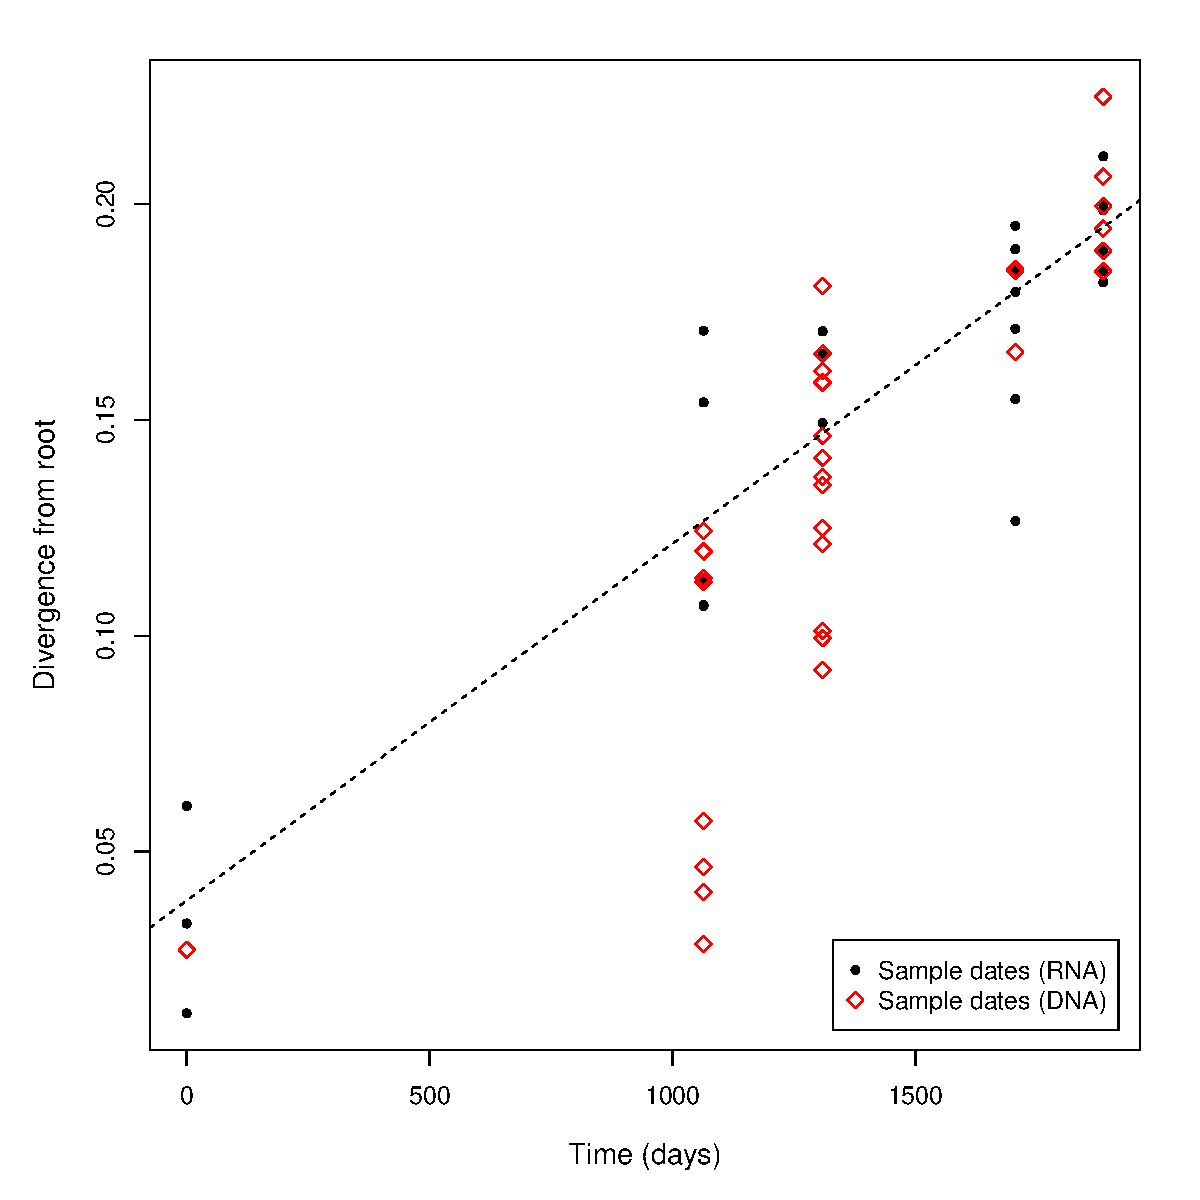
\includegraphics[width=8cm]{{figures/ancre.ogr}.pdf}
		\caption{Patient 2658 from the \emph{plasma} data set}
		\label{fig:resultsancre}
	\end{subfigure}
%	Patient: patient_1
	\begin{subfigure}[ht]{8cm}
		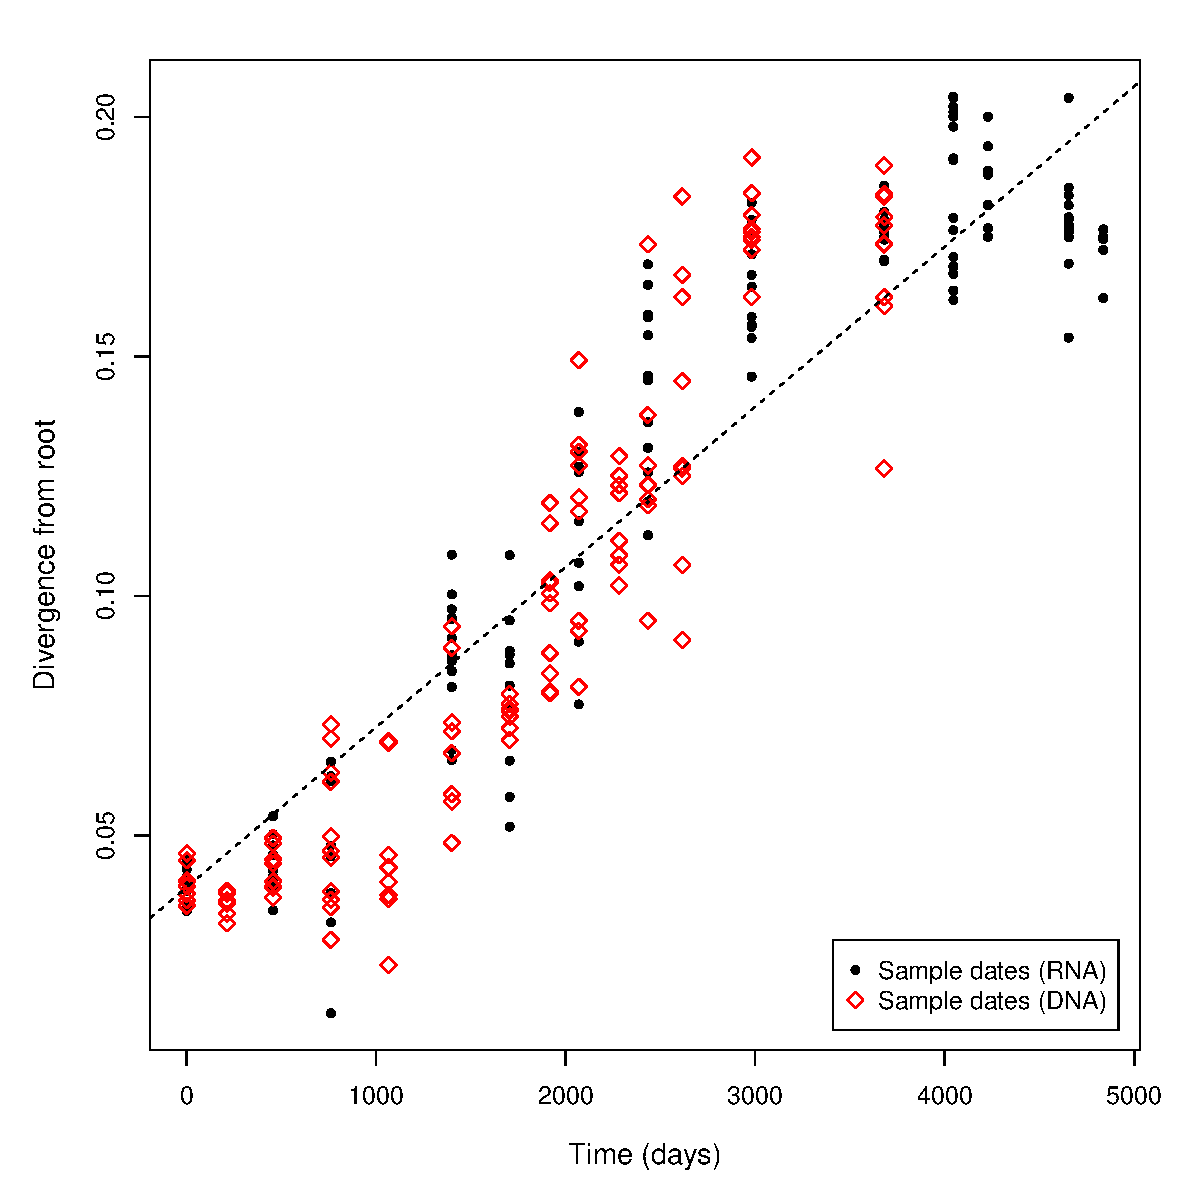
\includegraphics[width=8cm]{{figures/lanl.ogr}.pdf}
		\caption{Patient 13889 from the \emph{mixed} data set}
		\label{fig:resultslanl}
	\end{subfigure}
	\caption[Examples]{As Figure 4 from the primary work, except using outgroup rooting.}
	\label{fig:results2}
\end{figure}

\begin{figure}[ht]
	\centering
	\begin{subfigure}[ht]{8cm}
		\centering
		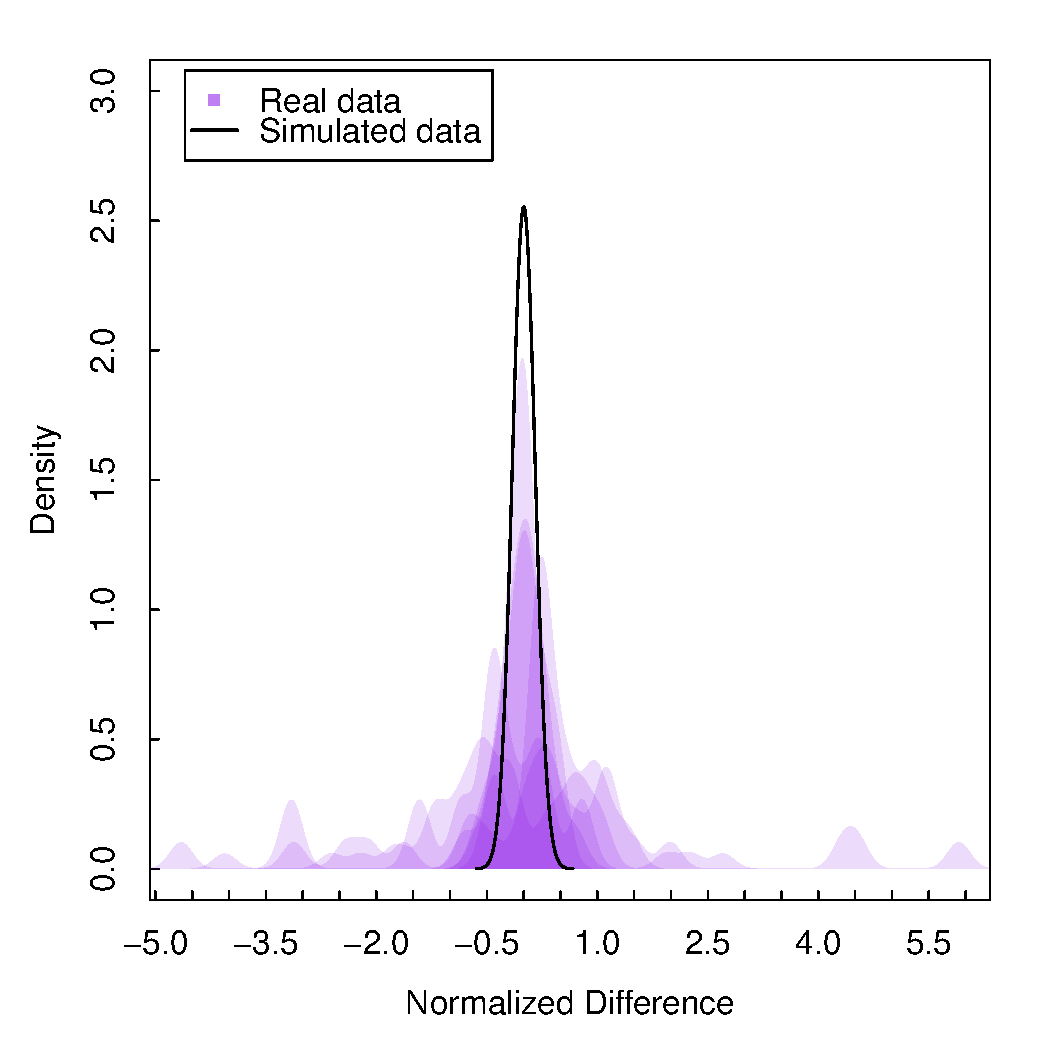
\includegraphics[width=8cm]{{figures/ancre.hist.ogr}.pdf}
		\caption{Density of the scaled difference of the \emph{plasma} data set with a solid line representing the density of the difference of the simulated data set without latency.}
		\label{fig:densityancre}
	\end{subfigure}
	\begin{subfigure}[ht]{8cm}
		\centering
		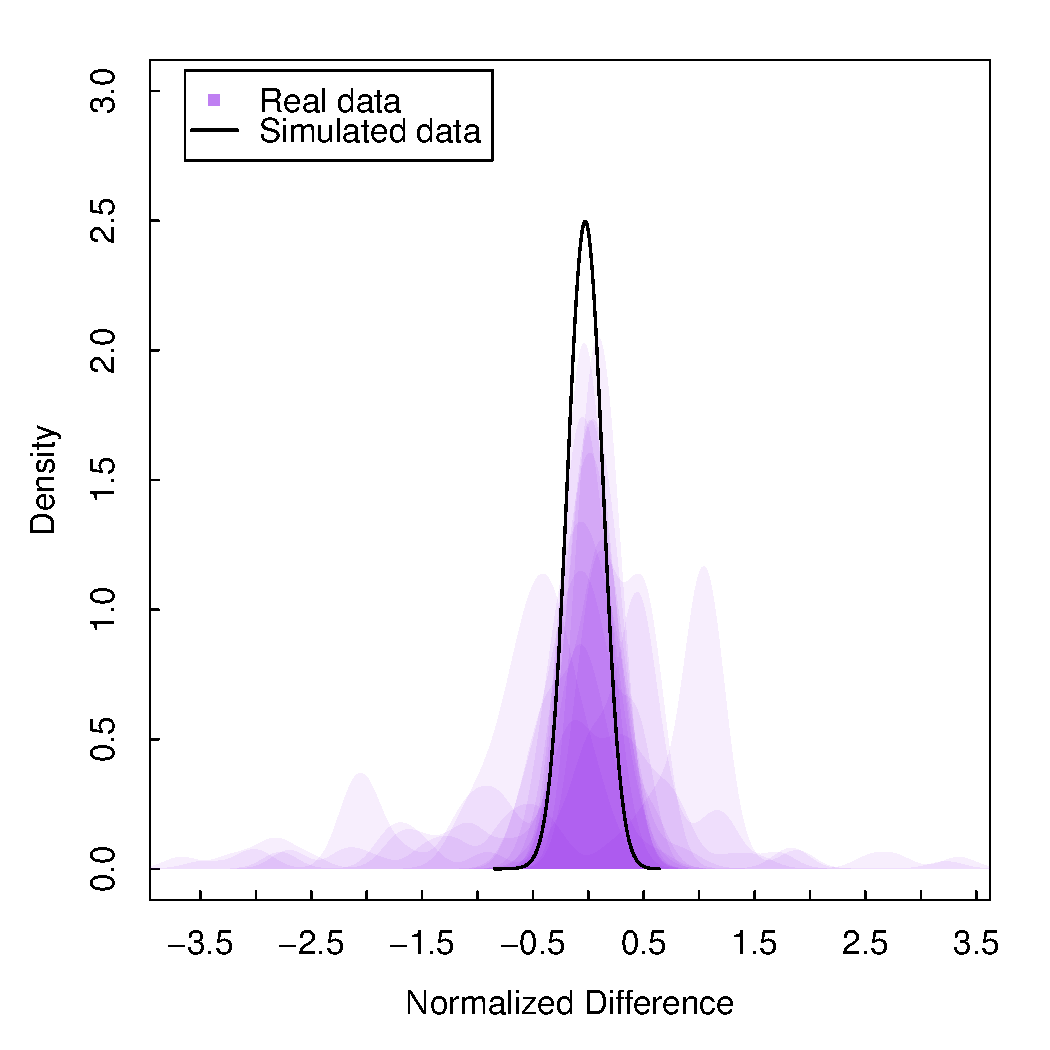
\includegraphics[width=8cm]{{figures/lanl.hist1.ogr}.pdf}
		\caption{Density of the scaled difference of the \emph{plasma} data set with a solid line representing the density of the scaled difference of the first set of simulated data set with latency.}
		\label{fig:densitylanl}
	\end{subfigure}
\begin{comment}
	\begin{subfigure}[ht]{8cm}
		\centering
		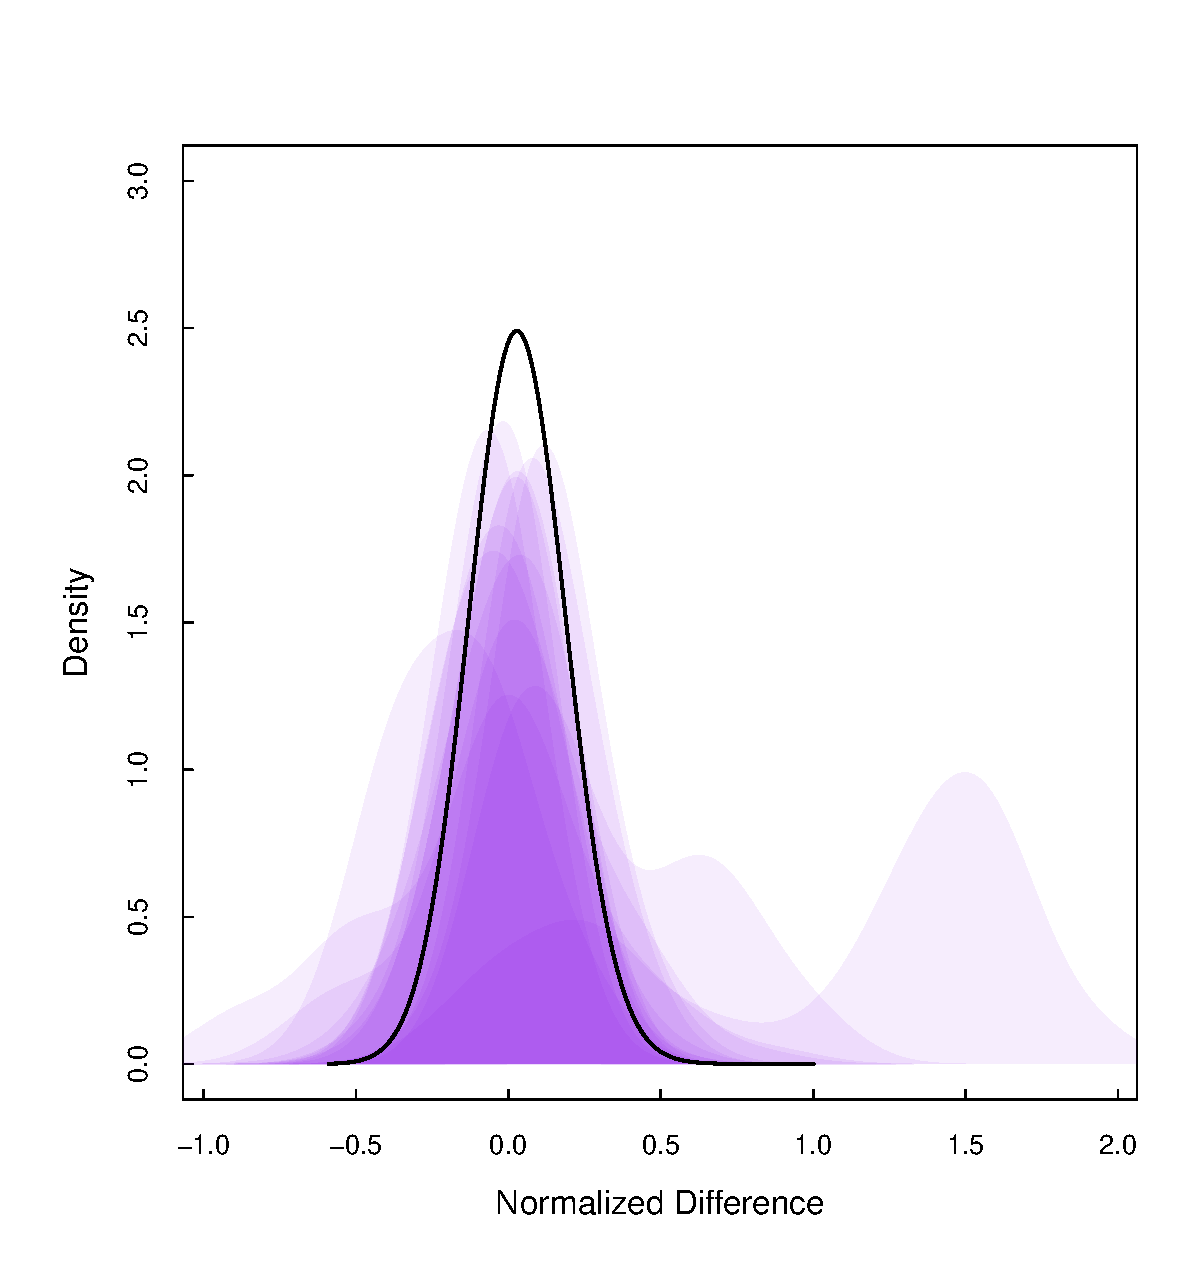
\includegraphics[width=8cm]{{figures/lanl.hist2}.pdf}
		\caption{Density of the scaled difference of the \emph{plasma} data set with a solid line representing the density of the scaled difference of the second set of simulated data set with latency.}
		\label{fig:densitylanl2}
	\end{subfigure}
\end{comment}
	\caption[Difference Density]{As Figure 5 from the primary work, except using outgroup rooting.}
	\label{fig:density}
\end{figure}

\begin{figure}[ht]
	\centering
	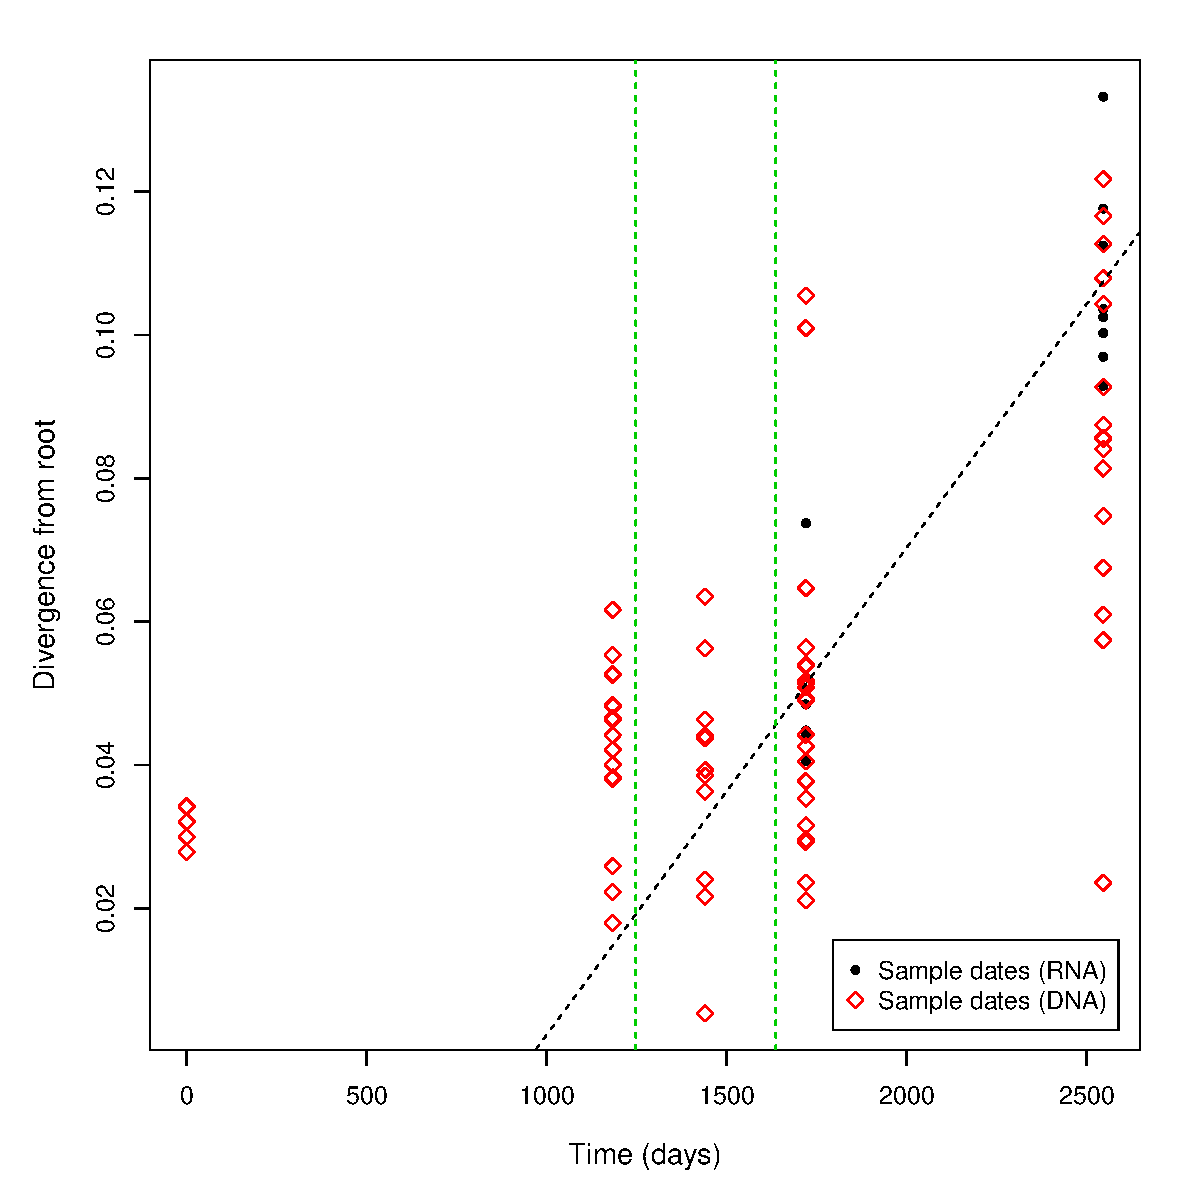
\includegraphics[width=12cm]{{figures/patient_16617.ogr}.pdf}
	\caption{As Figure 6 from the primary work, except using outgroup rooting}
	\label{fig:treatment}
\end{figure}

% Tables
\begin{table*}[!ht]
\def\arraystretch{1.3}%
\begin{center}
\begin{tabular}{lrrrr} 
Patient ID & $p$-value & Median Difference (days) & RMSD (days) & Scaled RMSD \\ 
\hline
\badpat{825 & $0.52$ & $1.1 \times 10^3$ & $6.8 \times 10^3$ & 2.3} \\
2658 & $< 2.2 \times 10^{-15}$  & -67. & 380 & 0.20 \\
\badpat{7259 & $0.285$ & -7.70 & $1.2 \times 10^{3}$ & 1.3} \\
\badpat{7263 & $0.074$ & -25. & 200 & 0.78} \\
\badpat{7265 & $0.030$ & -110 & 320 & 1.2} \\
13333 & $2.4 \times 10^{-8}$ & 28. & 160 & 0.31 \\
13334 & $5.8 \times 10^{-10}$ & 22. & 210 & 0.29 \\
13336 & $9.9 \times 10^{-3}$ & 220 & 470 & 0.63 \\
\badpat{35566 & $0.016$ & 75. & 320 & 1.2} \\
\hline
820 & $4.8 \times 10^{-4}$ & $-1.3 \times 10^{3}$ & $1.7 \times 10^{3}$ & 0.56 \\
821 & $< 2.2 \times 10^{-15}$ & -120. & 550 & 0.23 \\
822 & $2.0 \times 10^{-15}$ & 130 & 690 & 0.32 \\
824 & $< 2.2 \times 10^{-15}$ & -9.1 & 600 & 0.19 \\
\badpat{10137 & $0.031$ & 810 & 900 & 0.32} \\
10138 & $< 2.2 \times 10^{-15}$ & -72. & 610 & 0.18 \\
\badpat{10586 & $0.45$ & $5.2 \times 10^3$ & $7.8 \times 10^{3}$ & 1.7} \\
13889 & $< 2.2 \times 10^{-15}$ & -150 & 640 & 0.13 \\
\badpat{34391 & 0.056 & -33 & 280 & 0.76} \\
\badpat{34393 & 0.47 & 340 & 400 & 1.1} \\
\badpat{34396 & 0.59 & -690 & 970 & 2.9} \\
34399 & $< 2.2 \times 10^{-15}$ & 29 & 250 & 0.17 \\
\badpat{34408 & 0.75 & $-2.1 \times 10^{3}$ & $1.1 \times 10^{4}$ & 21.} \\
34410 & $2.3 \times 10^{-3}$ & -16. & 590 & 1.3 \\
\badpat{34411 & 0.39 & 210. & 410 & 0.89} \\
10769 & $4.3 \times 10^{-5}$ & -530 & $2.5 \times 10^3$ & 1.3 \\
16616 & $1.9 \times 10^{-6}$ & -100 & 800 & 0.31 \\
16617 & $1.0 \times 10^{-7}$ & 75. & 550 & 0.22 \\
16618 & $7.7 \times 10^{-12}$ & 180 & 350 & 0.15 \\
16619 & $5.5 \times 10^{-4}$ & 480 & 730 & 0.36 \\
\hline
\end{tabular}
\end{center}
  \caption{Details of the linear models applied to the real data sets using outgroup rooting. RMSD is the root mean squared deviance. Patients where we were unable to reject the null hypothesis are marked in red.
   }\label{tab:patientserrorogr} 
\end{table*}

\end{document}

